\chapter{Instrument response and units}\label{ch:response}

\section{Why counts are not ground motion}
A record in counts mixes two things: the ground motion and the way the instrument responds to it. The same ground
velocity at 0.1~Hz and at 10~Hz produces very different counts, because a geophone responds weakly below its natural
frequency. To compare records from different instruments, or to report ground velocity, the instrument's effect must
be removed. This is done with the \emph{instrument response}.

\section{Linear systems and the transfer function}
Over its operating range a seismometer behaves as a linear, time-invariant system. If the ground velocity is
$v(t)$ and the digitised output is $d(t)$ (in counts), then in the frequency domain
\begin{equation}
  D(f) = T(f)\,V(f),
\end{equation}
where $V$ and $D$ are the Fourier transforms of $v$ and $d$ and $T(f)$ is the complex \emph{transfer function}, in
counts per (m/s). Its magnitude $\abs{T}$ says how much each frequency is amplified; its phase says how much it is
delayed.

\subsection{A geophone as a second-order system}
The mechanical part of a geophone is a damped oscillator. With natural angular frequency
$\omega_0 = 2\pi f_0$ and fractional damping $h$ the velocity transfer function in the Laplace variable
$s=\jj\omega$ is
\begin{equation}\label{eq:geophone}
  T_g(s) = G\,\frac{s^{2}}{s^{2} + 2h\,\omega_0\,s + \omega_0^{2}},
\end{equation}
where $G$ is the generator constant (volts per m/s) in the flat band. Equation~\eqref{eq:geophone} has two zeros at
$s=0$ and two poles at $s=\omega_0\bigl(-h \pm \jj\sqrt{1-h^2}\bigr)$. \Cref{fig:response} shows its magnitude and
phase for $f_0 = 4.5$~Hz.

\begin{figure}[tbp]
\centering
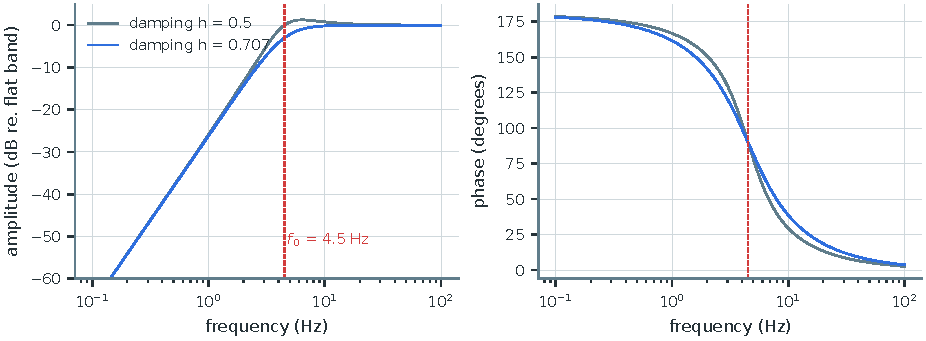
\includegraphics[width=\linewidth]{theory-response}
\caption{Magnitude and phase of the velocity response~\eqref{eq:geophone} of a 4.5~Hz geophone for two damping
values. Illustrative only: the real response of a given Shake comes from its StationXML file.}\label{fig:response}
\end{figure}

Three properties matter for what follows.
\begin{enumerate}
\item \textbf{Flat above $f_0$.} For $f\gg f_0$, $T_g\to G$: the output follows ground velocity directly.
\item \textbf{Falling as $f^{2}$ below $f_0$.} The double zero at the origin makes the response fall at 40~dB per
  decade (a factor 100 in amplitude for each factor 10 in frequency).
\item \textbf{Zero at $f=0$.} A constant (DC) input produces no output from the mechanical part.
\end{enumerate}

\subsection{The complete chain}
The digitiser adds its own stages: amplification, a digital anti-alias filter and decimation. The \emph{overall}
response is the product of the stage responses. Standards describe it as poles, zeros and a normalisation, and
distribute it as \emph{StationXML}. In the flat band the overall response reduces to a single number, the
\emph{sensitivity} $\Lambda$ in counts per m/s.

\section{Removing the response}
Estimating the ground velocity means dividing by $T$ in the frequency domain:
\begin{equation}\label{eq:deconv}
  \hat v(t) = \mathcal{F}^{-1}\!\left[\frac{D(f)}{T(f)}\right].
\end{equation}
Equation~\eqref{eq:deconv} hides a numerical trap. Below $f_0$, $\abs{T}$ becomes very small, so dividing by it
\emph{amplifies} whatever is there, which is mostly noise, and at $f=0$ the division is by zero. Practical
implementations therefore (i) remove the mean first, (ii) taper the record so that its ends do not create
discontinuities, and (iii) limit the division with a \emph{water level}: wherever $\abs{T}$ falls below a chosen
fraction of its maximum, it is replaced by that fraction.

\begin{rs3dapp}
The \ui{counts}/\ui{m/s} switch calls ObsPy's \code{remove\_response(inventory, output="VEL")} in
\file{core/export.py}, with ObsPy's defaults, which were read from the installed library: zero-mean removal on, a
5\,\% cosine taper, a water level of 60~dB, and no pre-filter. The response is a StationXML file downloaded once from
the Raspberry Shake FDSN web service and cached in the data folder (\file{core/response.py}); with the file cached
the switch works offline. Without a cached response and without Internet the Data page reports the error, and the Helicorder page
reports it and returns to counts instead of showing an empty chart.
\end{rs3dapp}

\begin{rs3dwarn}[Velocity below the natural frequency]
Because the response is deconvolved with a water level, ground velocity at frequencies well below
4.5~Hz is only as reliable as the signal-to-noise ratio there. Long-period phenomena, such as the ocean microseism near
0.2~Hz or the surface waves of distant earthquakes, are recoverable but noisier than the same signal on a broadband
sensor.
\end{rs3dwarn}

\section{The DC offset}
Raw counts almost never oscillate around zero. Electronic offsets in the sensor and ADC add a constant,
typically thousands of counts for a Shake. Because $T(0)=0$, such a constant is \emph{not} ground motion, and any
processing that does not remove it has to cope with it:

\begin{itemize}
\item \textbf{Spectra.} An offset leaks into the lowest bins and, through window sidelobes, into higher ones.
  The application subtracts the mean before every spectrum (Chapter~\ref{ch:spectral}).
\item \textbf{Filtering.} The filter route removes the mean before filtering (\code{detrend("demean")} in
  \file{core/export.py}).
\item \textbf{The helicorder.} Plotting raw counts would shift every row by the offset and dominate the amplitude
  scale (\cref{fig:dcoffset} in Chapter~\ref{ch:vis}); each row therefore has its median removed.
\end{itemize}

\begin{rs3dkey}
Counts are an instrument-dependent integer with an arbitrary offset. Ground velocity needs the response; every
display that does not use it must at least remove the mean.
\end{rs3dkey}
